\documentclass[11pt,a4paper]{article}
\usepackage[T1]{fontenc}
\usepackage[margin=2.3cm]{geometry}
\usepackage{amsmath,amssymb}
\usepackage{graphicx}
\usepackage[dvipsnames]{xcolor}
\usepackage{enumitem}
\usepackage[colorlinks=true,linkcolor=blue,urlcolor=blue]{hyperref}
\setlength{\parskip}{0.6em}
\setlength{\parindent}{0pt}
\begin{document}

\begin{center}{\LARGE\bfseries openportfolio}\\[0.4em]{\large See why a mix of assets is steadier than any one of them, in three sessions.}\\[0.2em]\small PAN IIT OSS explainer \textbullet{} secondary school to diploma / undergraduate (levels 3-5)\end{center}

\section*{Why this exists}
Why is a mix of assets steadier than any one of them? This explainer shows the mathematics behind diversification: average, risk, correlation and the covariance matrix, using only simple algebra and a few matrix products. All data are synthetic and made up.

\section*{The end goal}
See how diversification lowers risk in a portfolio. The end goal is to see how diversification lowers risk in a portfolio, and where it stops: the part of risk that all assets share, the surprising effect of rising correlations, and the unreliability of weights computed from a short history. This is general education, not investment advice.

\section*{How the three sessions build up}
\begin{enumerate}[nosep]
\item \textbf{Session 1: Do not put all your eggs in one basket} (Level 1, conceptual interactive model, 60 min).
\item \textbf{Session 2: Return, risk and correlation of two assets} (Level 2, mathematical engineering model, 75 min).
\item \textbf{Session 3: Many assets, the efficient frontier and its limits} (Level 3, simulation and validation, 90 min).
\end{enumerate}

\section{Session 1: Do not put all your eggs in one basket}

\subsection*{A. Real-world problem}
You have some savings to put into a small business. One shop sells umbrellas, the other ice cream. On rainy days the umbrella shop earns a lot and the ice cream shop little; on dry days it is the other way round. Put everything in one shop and your income jumps with the weather. Put some in each and the two shops cover for each other. How much steadier does it get, and what is the best split? This is a toy model for learning, general education only, not investment advice: the shops and incomes are made up, and real markets do not behave like a coin flip of weather.

\subsection*{B. Concept and theory}
Each day is rainy with chance p = 0.5 or dry. With all the money in the umbrella shop the income is 100 on a rainy day and 20 on a dry day; with all the money in the ice cream shop it is 30 and 90 (made-up money units per day). If a fraction f of the money goes into the umbrella shop and 1 - f into the ice cream shop, the income is the same split of the two: f times the umbrella income plus (1 - f) times the ice cream income. The average income is the average over the days. The swing is the standard deviation: the typical distance of a day from the average. Because there are only two kinds of day, the swing is the gap between the rainy-day and dry-day income times the square root of p (1 - p). A small swing means a steady income.

\begin{itemize}[nosep]
\item f: fraction of the money in the umbrella shop (no unit (0 to 1))
\item p: chance that a day is rainy (no unit (0 to 1))
\item R, D: income on a rainy day, on a dry day (money units per day)
\item average: average daily income (money units per day)
\item swing: standard deviation of the daily income (money units per day)
\end{itemize}

\begin{equation*}
R(f)=100f+30(1-f),\qquad D(f)=20f+90(1-f)
\end{equation*}

\begin{equation*}
\text{average}=pR+(1-p)D,\qquad \text{swing}=|R-D|\sqrt{p(1-p)}
\end{equation*}

\begin{equation*}
\text{swing}=|70f-30|\quad(p=0.5),\qquad \text{zero swing at } f=\tfrac{3}{7}
\end{equation*}

\begin{center}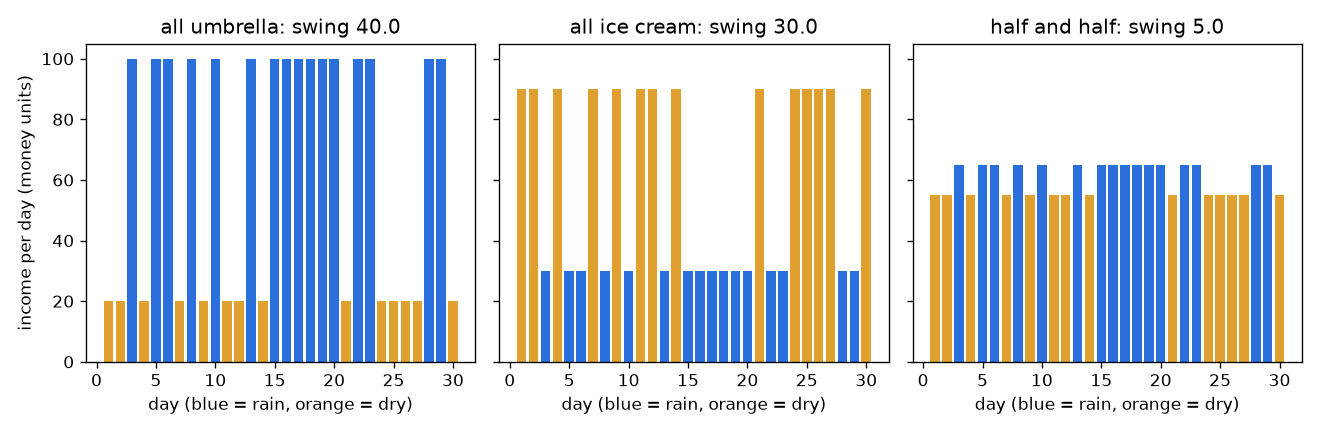
\includegraphics[width=0.85\linewidth]{figures/s01_shop_incomes.png}\\\small 30 days of income: one shop jumps between low and high; half and half is almost flat.\end{center}

\subsection*{E. Worked example}
Put half the money in each shop. Find the income on a rainy day and on a dry day, the average income and the swing.
\begin{enumerate}[nosep]
\item Rainy day: 0.5 * 100 + 0.5 * 30 = 65 money units.
\item Dry day: 0.5 * 20 + 0.5 * 90 = 55 money units.
\item Average = 0.5 * 65 + 0.5 * 55 = 60 money units per day (the same as either shop alone).
\item Swing = \textbar{}65 - 55\textbar{} * sqrt(0.5 * 0.5) = 10 * 0.5 = 5 money units per day.
\item Compare: all umbrella has swing \textbar{}100 - 20\textbar{} * 0.5 = 40 and all ice cream has \textbar{}30 - 90\textbar{} * 0.5 = 30.
\end{enumerate}
\textbf{Answer.} Half and half gives 65 on a rainy day, 55 on a dry day, average 60 and swing 5, against swings of 40 and 30 for a single shop. The checkpoint also confirms it with 365 seeded days: 189 rainy days and swings 40.0, 30.0 and 5.0.

\subsection*{F. Questions}
\begin{enumerate}[nosep]
\item \textbf{Conceptual.} Why does putting money in both shops make the income steadier, even though each shop is unsteady?
\item \textbf{Numerical.} Put 25 percent of the money in the umbrella shop. Find the rainy-day income, the dry-day income, the average and the swing (rain chance 0.5).
\item \textbf{Graph and simulation interpretation.} In the graph of swing against split, where is the swing zero and what are the swings at 0 and at 100 percent? What does the V shape mean on each side of the bottom?
\item \textbf{Design and optimisation challenge.} Design: you want the swing to be at most 10 money units per day. Which splits work? Why might you not choose exactly the zero-swing split?
\end{enumerate}

\section{Session 2: Return, risk and correlation of two assets}

\subsection*{A. Real-world problem}
Session 1 had shops that were exactly opposite. Real assets are only partly opposite, so we need numbers: what an asset earns on average (mean return), how much it wobbles (standard deviation, our measure of risk) and how much two assets move together (correlation rho, between -1 and +1). Then the question: how should we split money between two assets to get the least risk, or the best risk for a return we want? All assets here are synthetic and their returns made up (asset 1: mean 10 percent, risk 20 percent; asset 2: mean 6 percent, risk 10 percent per year). This is general education, not investment advice, and a model like this does not predict real markets.

\subsection*{B. Concept and theory}
Yearly returns are drawn from a seeded generator: r1 = mu1 + s1 z1 and r2 = mu2 + s2 (rho z1 + sqrt(1 - rho\textasciicircum{}2) z2), where z1 and z2 are independent bell-curve numbers. The means are mu1, mu2, the risks (standard deviations) are s1, s2 and the correlation is rho. With weight w in asset 1 and 1 - w in asset 2, the expected return is a weighted average, but the variance has a cross term that depends on rho. For rho = 1 the variance is (w s1 + (1 - w) s2)\textasciicircum{}2, so risk is just the weighted average of the risks: no benefit. For rho = -1 it is (w s1 - (1 - w) s2)\textasciicircum{}2, which is zero at w = s2 / (s1 + s2). The weight with the least variance comes from setting the derivative to zero. For other inputs it can fall outside 0 to 1, which would mean borrowing or short selling.

\begin{itemize}[nosep]
\item mu1, mu2: mean (expected) yearly return of each asset (fraction per year (0.10 = 10\%))
\item s1, s2: risk: standard deviation of the yearly return (fraction per year)
\item rho: correlation of the two returns (no unit, from -1 to 1)
\item w: weight (fraction of money) in asset 1 (no unit)
\item w*: weight with the least variance (no unit)
\end{itemize}

\begin{equation*}
E[R_p]=w\mu_1+(1-w)\mu_2
\end{equation*}

\begin{equation*}
\sigma_p^2=w^2\sigma_1^2+(1-w)^2\sigma_2^2+2w(1-w)\rho\sigma_1\sigma_2
\end{equation*}

\begin{equation*}
\rho=-1:\ \sigma_p=|w\sigma_1-(1-w)\sigma_2|=0\ \Rightarrow\ w=\frac{\sigma_2}{\sigma_1+\sigma_2}
\end{equation*}

\begin{equation*}
w^*=\frac{\sigma_2^2-\rho\sigma_1\sigma_2}{\sigma_1^2+\sigma_2^2-2\rho\sigma_1\sigma_2}
\end{equation*}

\begin{center}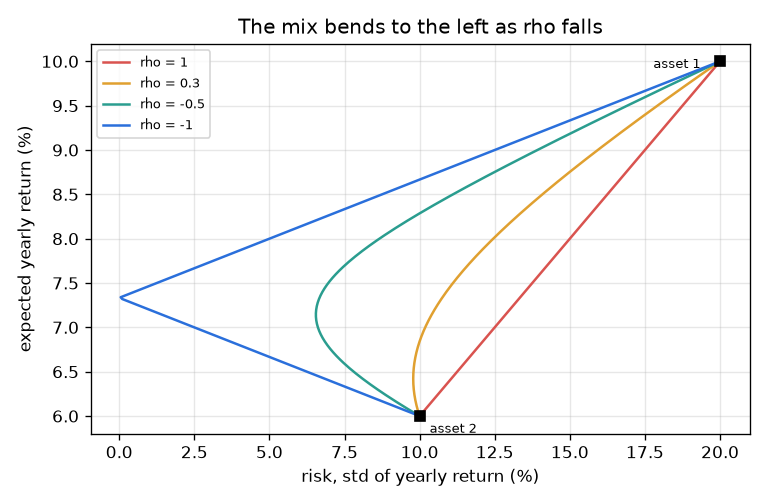
\includegraphics[width=0.85\linewidth]{figures/s02_risk_return_curves.png}\\\small Risk-return curve of the mix; it bends left as correlation falls.\end{center}

\subsection*{E. Worked example}
Put half the money in each asset (w = 0.5) with correlation rho = 0.3. Find the expected return, the variance and the risk, and check against a simulated portfolio of 100000 years.
\begin{enumerate}[nosep]
\item Expected return = 0.5 * 0.10 + 0.5 * 0.06 = 0.08, that is 8 percent.
\item Variance = 0.25 * 0.04 + 0.25 * 0.01 + 2 * 0.25 * 0.3 * 0.2 * 0.1 = 0.0100 + 0.0025 + 0.0030 = 0.0155.
\item Risk = sqrt(0.0155) = 0.1245, that is 12.45 percent.
\item Simulation (seed 7, 100000 years, correlation 0.3): the sampled portfolio has mean 0.0800 and risk 0.1245. They agree.
\item Compare with the single assets: 20 percent and 10 percent. The mix has an average return of 8 percent with less than the average of the two risks (15 percent).
\end{enumerate}
\textbf{Answer.} Return 8.00 percent, variance 0.0155, risk 12.45 percent; the simulation gives 0.0800 and 0.1245. For the exact version, the checkpoint also shows that the formula is an identity when built from the sample variances and covariance.

\subsection*{F. Questions}
\begin{enumerate}[nosep]
\item \textbf{Conceptual.} Why does a correlation of +1 give no diversification benefit, while a correlation of -1 can remove the risk completely?
\item \textbf{Numerical.} Assets 1 and 2 are uncorrelated (rho = 0). Find the weight with the least risk, that risk, and the expected return there.
\item \textbf{Graph and simulation interpretation.} In the first figure, at rho = 0.3 where is the minimum of the risk curve, and is it lower than the risk of the safer asset (10 percent)? What would happen at rho = 1?
\item \textbf{Design and optimisation challenge.} Design: you want an expected return of at least 8 percent and a risk of at most 11 percent from these two assets. What weight do you need and how low must the correlation be? Is rho = 0.3 enough? What can you do if not?
\end{enumerate}

\section{Session 3: Many assets, the efficient frontier and its limits}

\subsection*{A. Real-world problem}
A real portfolio may hold dozens of assets. If I keep adding assets, does my risk go to zero? Among all mixes of several assets, which has the least risk for the return I want, and which gives the best return per unit of risk? And all of this is computed from numbers estimated from a short history: how much should I trust it? Everything here is synthetic (four made-up assets, a made-up risk-free rate), general education only, not investment advice. A model like this does not predict real markets: real returns have fatter tails and correlations change, especially in a crisis.

\subsection*{B. Concept and theory}
For N assets with equal weights 1/N, common risk s and common correlation rho, the variance is s\textasciicircum{}2 (1/N + (1 - 1/N) rho). The first part, s\textasciicircum{}2 / N, is the idiosyncratic risk and vanishes as N grows; the second tends to s\textasciicircum{}2 rho, the market risk shared by all, which no number of assets removes. With several assets, the covariance matrix Sigma holds every variance and covariance and the portfolio variance is w' Sigma w. Minimising it for a target return m with weights summing to 1 has a closed form (Lagrange multipliers); the set of these portfolios is the efficient frontier. The Sharpe ratio (return minus the risk-free rate, divided by risk) is largest for the tangency portfolio with weights proportional to the inverse of Sigma times (mu - rf). The same formulas applied to estimates from a short history give weights that look better in-sample than they really are.

\begin{itemize}[nosep]
\item N: number of assets (no unit)
\item s, rho: common risk and correlation (equal-weight case) (fraction per year, no unit)
\item mu: vector of mean returns (fraction per year)
\item Sigma: covariance matrix (variances on the diagonal) (fraction\textasciicircum{}2 per year)
\item w: vector of weights, summing to 1 (no unit)
\item rf: risk-free rate (made up: 0.02) (fraction per year)
\item T: number of periods in the history used for estimates (periods)
\end{itemize}

\begin{equation*}
\sigma_p^2=\sigma^2\left(\frac1N+\Big(1-\frac1N\Big)\rho\right)\ \longrightarrow\ \sigma^2\rho\quad(N\to\infty)
\end{equation*}

\begin{equation*}
A=\mathbf 1^{\mathsf T}\Sigma^{-1}\mathbf 1,\ B=\mathbf 1^{\mathsf T}\Sigma^{-1}\mu,\ C=\mu^{\mathsf T}\Sigma^{-1}\mu,\ D=AC-B^2
\end{equation*}

\begin{equation*}
w(m)=\Sigma^{-1}(\lambda\mathbf 1+\gamma\mu),\ \lambda=\frac{C-Bm}{D},\ \gamma=\frac{Am-B}{D},\qquad \sigma^2(m)=\frac{Am^2-2Bm+C}{D}
\end{equation*}

\begin{equation*}
\text{Sharpe}=\frac{\mu_p-r_f}{\sigma_p},\qquad w_{\tan}=\frac{\Sigma^{-1}(\mu-r_f\mathbf 1)}{\mathbf 1^{\mathsf T}\Sigma^{-1}(\mu-r_f\mathbf 1)}
\end{equation*}

\begin{center}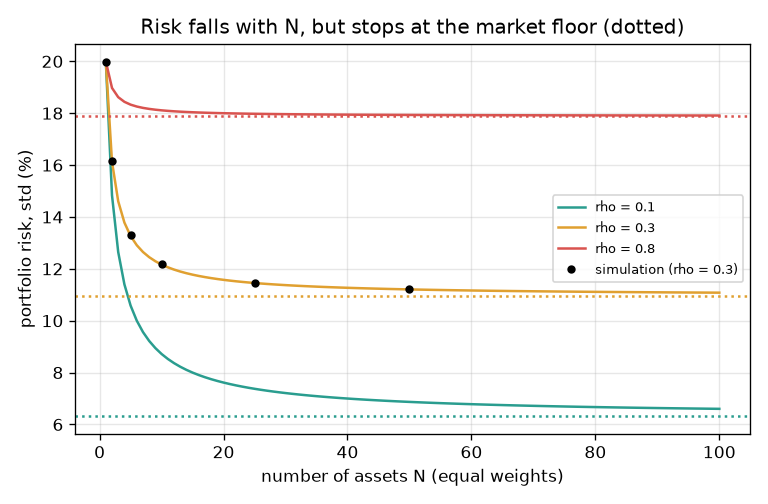
\includegraphics[width=0.85\linewidth]{figures/s03_diversification_vs_n.png}\\\small Risk against N for three correlations: it falls, then flattens at the market floor (dotted); dots are simulated.\end{center}

\subsection*{E. Worked example}
Four assets, each with risk 0.20 and common correlation 0.3, held with equal weights. Find the portfolio variance and risk, and the limit as the number of assets grows.
\begin{enumerate}[nosep]
\item Variance = 0.04 * (1/4 + (3/4) * 0.3) = 0.04 * (0.25 + 0.225) = 0.04 * 0.475 = 0.0190.
\item Risk = sqrt(0.0190) = 0.1378, that is 13.78 percent, about 31 percent below the 20 percent of one asset.
\item Limit: s * sqrt(rho) = 0.2 * sqrt(0.3) = 0.1095, that is 10.95 percent. Even a million assets stay above it.
\item Check by simulation: 200000 years of one-factor returns give 0.1380 for N = 4 (the formula gives 0.1378).
\end{enumerate}
\textbf{Answer.} Variance 0.0190, risk 13.78 percent for N = 4; the floor is 10.95 percent. The checkpoint also reproduces the formula from a covariance matrix.

\subsection*{F. Questions}
\begin{enumerate}[nosep]
\item \textbf{Conceptual.} Why can you never diversify away all the risk by adding more and more assets, if they share a common correlation?
\item \textbf{Numerical.} Find the variance and risk of an equal-weight portfolio of N = 10 assets with s = 0.20 and rho = 0.3. By what percent is it below the risk of one asset?
\item \textbf{Graph and simulation interpretation.} In the estimation-error figure, what is the predicted risk and the true risk for a history of T = 12 periods, and for T = 240? What does the gap tell you?
\item \textbf{Design and optimisation challenge.} Design: with s = 0.20 and rho = 0.3 you want a risk of at most 12 percent using equal weights. How many assets do you need? What if the assets had rho = 0.5? What does that say about a crisis?
\end{enumerate}

\section{Real-world mini-project}
\textbf{Build a four-asset synthetic portfolio and test it honestly.} Here is a made-up asset set B (education only, not advice). Yearly mean returns: 4\%, 7\%, 9\%, 13\%. Standard deviations: 8\%, 12\%, 18\%, 30\%. Correlations: 0.2 between assets 1 and 2, 0.1 between 1 and 3, 0 between 1 and 4, 0.3 between 2 and 3, 0.2 between 2 and 4, 0.6 between 3 and 4. The risk-free rate is 2\%. Use the Session 3 functions to: build the covariance matrix and check it is positive definite; find the minimum-variance weights and the Sharpe-best (tangency) weights using the true numbers; then draw a history of 36 yearly periods (draw\_sample with seed 21), estimate from it, and measure how the estimated minimum-variance portfolio really behaves. Repeat over 1000 histories with estimation\_experiment(36, 1000, mu, sigma, 21).

\section{The path ahead}
\begin{enumerate}[nosep]
\item \textbf{Session 4: Shrink the covariance estimate.} A function that mixes the sample covariance with a diagonal matrix, and a test over many seeded histories.
\item \textbf{Session 5: Stress-test the weights.} A stress function and a small search for weights that satisfy a return floor, a calm-risk cap and a stress-risk cap.
\item \textbf{Session 6: Equal risk contributions.} A solver for weights whose assets each carry the same share of the risk.
\item \textbf{Session 7: Fat tails.} A simulation with returns of the Student t type, scaled to the same standard deviation.
\end{enumerate}

\section{Answers and hints}

\subsection*{Session 1}
\begin{enumerate}[nosep]
\item \textbf{Conceptual.} Hint: Look at what each shop earns on a rainy day and on a dry day. Solution: The two shops are unsteady in opposite directions: when one earns a lot, the other earns little. Adding them makes the high days of one cover the low days of the other, so the total stays close to the same number. This only works because they move in opposite ways; two umbrella shops would rise and fall together and give no benefit.
\item \textbf{Numerical.} Hint: R = 100 f + 30 (1 - f) and D = 20 f + 90 (1 - f) with f = 0.25. Solution: R = 25 + 22.5 = 47.5 and D = 5 + 67.5 = 72.5 money units. Average = 0.5 * 47.5 + 0.5 * 72.5 = 60. Swing = \textbar{}47.5 - 72.5\textbar{} * 0.5 = 12.5, which matches \textbar{}70 * 0.25 - 30\textbar{} = 12.5. Sanity check: it lies between 5 (half and half) and 30 (all ice cream).
\item \textbf{Graph and simulation interpretation.} Hint: Set R = D, or read the bottom of the V. Solution: The swing is zero at f = 3/7 = 42.9 percent, where R = D. At 0 percent (all ice cream) it is 30 and at 100 percent (all umbrella) it is 40. Left of the bottom the ice cream shop dominates and the income is higher on dry days; right of the bottom the umbrella shop dominates and it is higher on rainy days. Either side, the swing grows because one shop's pattern wins.
\item \textbf{Design and optimisation challenge.} Hint: Solve \textbar{}70 f - 30\textbar{} \textless{}= 10. Solution: f must be between 2/7 = 28.6 percent and 4/7 = 57.1 percent. The zero-swing split 42.9 percent is the steadiest, but it depends on the made-up numbers being exactly right. If the shops' incomes or the rain chance change, the best split moves, so a split in the middle of the band is a safer choice. Trade-off: the average stays 60 for every split here, so steadiness is free; in real life lower risk often costs some average return (Session 2).
\end{enumerate}

\subsection*{Session 2}
\begin{enumerate}[nosep]
\item \textbf{Conceptual.} Hint: Look at the variance for rho = 1 and rho = -1: each is a perfect square. Solution: For rho = 1 the variance is (w s1 + (1 - w) s2)\textasciicircum{}2: the two wobbles always point the same way and add, so the risk is only the weighted average of the risks. For rho = -1 it is (w s1 - (1 - w) s2)\textasciicircum{}2: the wobbles point in opposite directions and subtract, and at w = s2 / (s1 + s2) they cancel exactly, leaving zero variance. Diversification works through the cross term 2 w (1 - w) rho s1 s2.
\item \textbf{Numerical.} Hint: w* = (s2\textasciicircum{}2 - 0) / (s1\textasciicircum{}2 + s2\textasciicircum{}2) with s1 = 0.20 and s2 = 0.10. Solution: w* = 0.01 / (0.04 + 0.01) = 0.2. Variance = 0.2\textasciicircum{}2 * 0.04 + 0.8\textasciicircum{}2 * 0.01 = 0.0016 + 0.0064 = 0.0080, so the risk is 0.0894 (8.94 percent), below both assets' 10 and 20 percent. Expected return = 0.2 * 0.10 + 0.8 * 0.06 = 0.068 (6.8 percent). Sanity check: the weight is small because asset 1 is the riskier one.
\item \textbf{Graph and simulation interpretation.} Hint: Find the dot of the matching colour and use w*. Solution: At rho = 0.3 the minimum is at w* = 0.1053 (about 10.5 percent in asset 1) with risk 9.79 percent: slightly below the safer asset's 10 percent, so a little of the riskier asset reduces the total risk. At rho = 1 the curve is a straight line, w* = -1 is outside 0 to 1, and the safest mix inside 0 to 1 is all asset 2 (risk 10 percent).
\item \textbf{Design and optimisation challenge.} Hint: w = 0.5 gives 8 percent. Solve the variance formula for rho with risk 0.11. Solution: A return of 8 percent needs w = 0.5 (it is a weighted average). With w = 0.5 the variance is 0.0125 + 0.01 rho; setting it to 0.11\textasciicircum{}2 = 0.0121 gives rho \textless{}= -0.04. So the assets must be slightly negatively correlated; rho = 0.3 (risk 12.45 percent) is not enough. Alternatives: accept a lower return, for example 7 percent needs w = 0.25 and gives a risk of 10.19 percent at rho = 0.3; or look for a third asset. Trade-off: return and risk move together, and the assumed rho may not be stable.
\end{enumerate}

\subsection*{Session 3}
\begin{enumerate}[nosep]
\item \textbf{Conceptual.} Hint: Split the variance into the part that shrinks like 1/N and the part that does not. Solution: Each asset's return is a shared (market) part plus its own part. Averaging many assets cancels their own parts (their variance falls like 1/N) but the shared part is the same in every asset, so averaging does not reduce it. The variance tends to s\textasciicircum{}2 rho, so the risk tends to s sqrt(rho). Only assets with a lower correlation (a different shared part) lower the floor.
\item \textbf{Numerical.} Hint: var = s\textasciicircum{}2 (1/N + (1 - 1/N) rho). Solution: Variance = 0.04 * (0.1 + 0.9 * 0.3) = 0.04 * 0.37 = 0.0148, so the risk is 0.1217 (12.17 percent). The reduction is (0.2 - 0.1217) / 0.2 = 39 percent. Sanity check: it lies between the floor 10.95 percent and the single-asset 20 percent.
\item \textbf{Graph and simulation interpretation.} Hint: Compare the two curves at each T; the dotted line is the best possible risk. Solution: At T = 12 the estimate predicts 0.0753 (7.53 percent) but the portfolio really has 0.1080 (10.80 percent), above the best possible 0.0914 (9.14 percent). At T = 240 they are 0.0906 and 0.0919, nearly equal. The gap shows that optimising on a short history overfits the noise: it picks weights that look safe in-sample but are worse out-of-sample, and more data (or simpler weights) reduces the problem.
\item \textbf{Design and optimisation challenge.} Hint: Solve 0.0144 \textgreater{}= 0.04 (1/N + (1 - 1/N) 0.3) for N, and compare 0.12 with the floor. Solution: 0.36 \textgreater{}= 0.3 + 0.7 / N gives N \textgreater{}= 11.7, so N = 12: risk 0.1197 (N = 11 gives 0.1206, just too high). With rho = 0.5 the floor is 0.2 * sqrt(0.5) = 0.1414 (14.14 percent), above 12 percent: no number of assets achieves it. In a crisis, correlations rise towards one and the floor rises, so a portfolio that met its target in calm times can miss it exactly when it matters. Trade-off: more assets cost more to hold and monitor.
\end{enumerate}

\section{How to join}
Read \texttt{CONTRIBUTING.md} in the repository, then pick an issue labelled \texttt{good first issue}. Repository: \url{https://github.com/KrunalPanchal1995/openportfolio}

\end{document}
